\documentclass{article}

\usepackage{geometry}
\usepackage{graphicx}
\usepackage{url}

\geometry{left=15mm, right=15mm, top=15mm, bottom=15mm}
\begin{document}
	
	\twocolumn \pagenumbering{gobble}
	
	{\centering\Large\bfseries REPORT: \normalfont Results of RPi-R Test\\ \normalsize\today \\ Raspberry Pi Rheometer v0.1.2\\}
	
	\vskip0.5cm \noindent
	{\centering\textbf{Introduction}\\}
	
	Here follows the results of the report generated on 28.06.17 at 14:54. This log is called ``280617''.
	
	Information logged by the RPi-R is plotted and summarised here, along with derived/calculated information.
	
	First plotted is the speed of rotation with respect to time, verifying the control system is working and the strain rate is being set properly. Second, the rheometry (normalised signal) is plotted against time. Third, the raw, corrected, and filtered piezo signals are plotted. Finally, the piezo, speed, and viscometry (filtered) signals are plotted against time.
	
	Below each plot is a discussion of the expected trends in the data.
	
	\vskip0.25cm \noindent
	{\centering\textbf{Plots}\\}
	
	{\centering 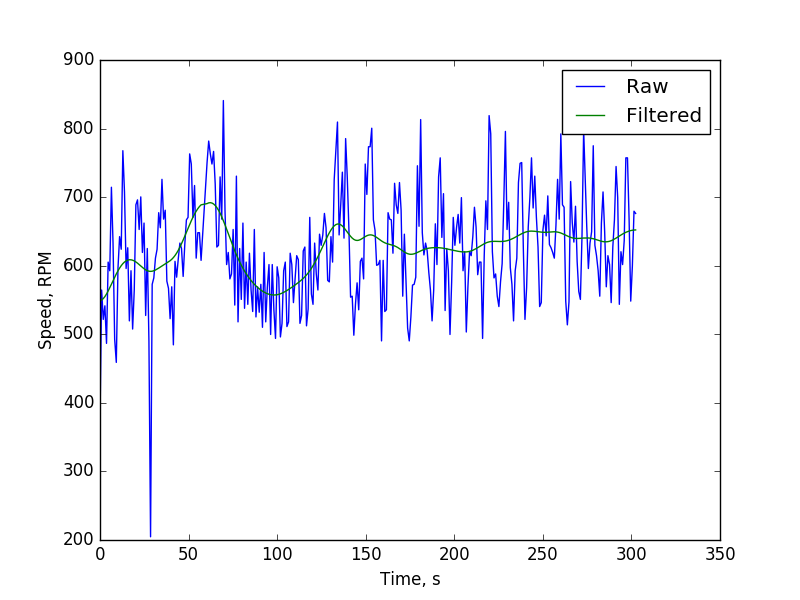
\includegraphics[width=0.4\textwidth]{strain_check.png}\\
	\textit{FIG. 1. Speed Check Plot}\\}

	Strain rate is set and controlled and so should follow function was set in the program - usually a straight line. There may be some low frequency noise in the beginning due to the motor just recently being turned on, or it could be the gearing acting up. Sudden dips not in the filtered signal are probably noise. Sudden dips that don't appear in the filtered signal, but do not match the rest of the noise are probably jamming events that have been filtered out. This would indicate a requirement to refine the filter function.

	{\centering 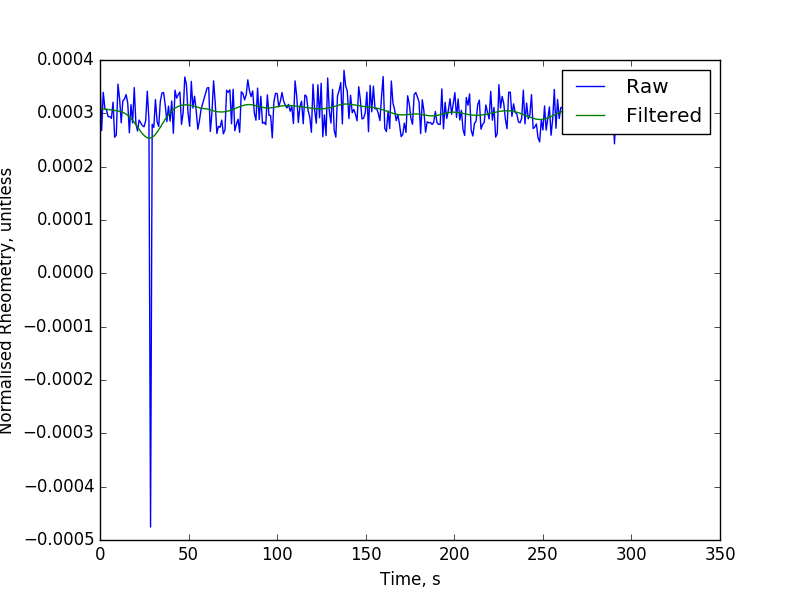
\includegraphics[width=0.4\textwidth]{viscometry.png}\\
	\textit{FIG. 2. Normalised Rheometry Plot}\\}

	The shape of this curve relies entirely on the material. Newtonian fluids have viscosity irrespective of the time, but other types may have some time dependence. The normalised rheometry signal only give a rough qualitative indication of what is happening to the rheology of the fluid.
	
	{\centering 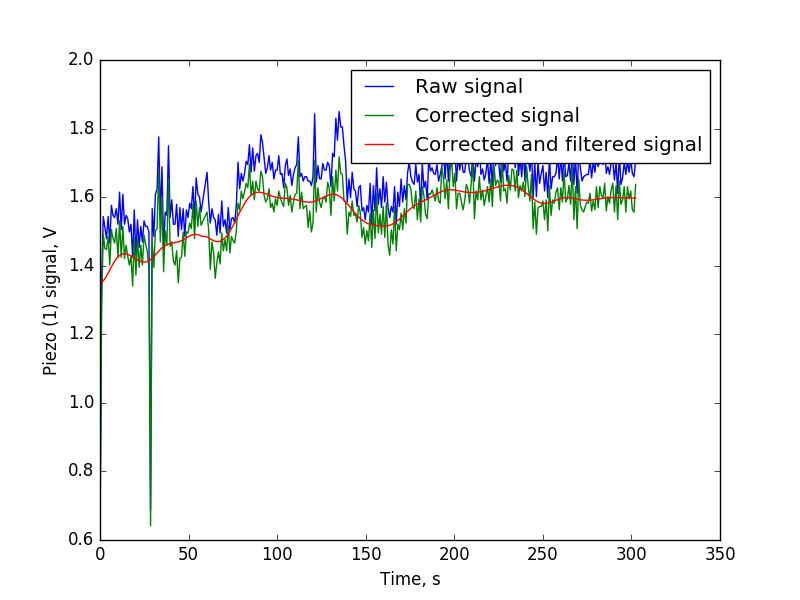
\includegraphics[width=0.4\textwidth]{general_piezo.png}\\
	\textit{FIG. 3. Raw and Corrected Piezo Plot}\\}

	This plot should, in theory, match up with the viscosity curve. Noise present in the signal here is mostly a combination of two things: literal noise from the motor transmitted through the fluid, through the probe, to the piezo plate (which acts as a microphone), as well as small variances in the regulated voltage reference used by the ADC --- this is removed in the ``corrected'' signal.
	
	\onecolumn
	
	{\centering 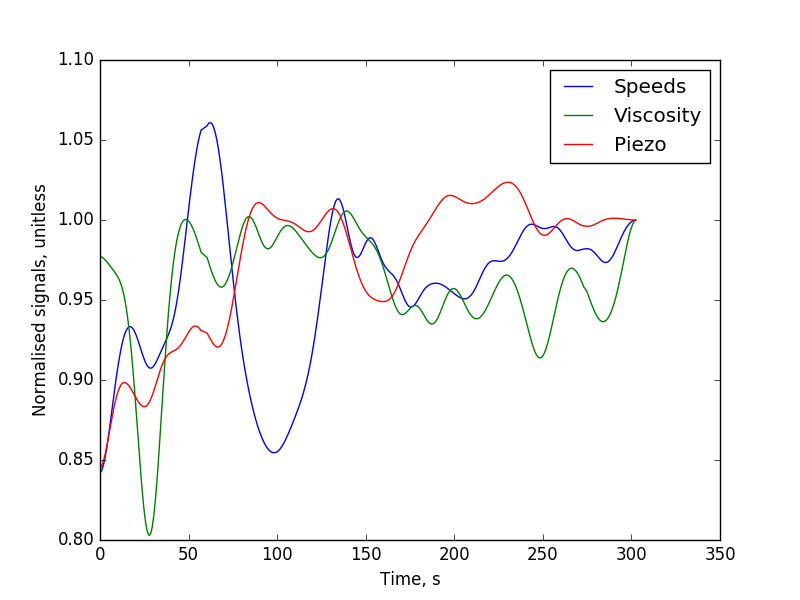
\includegraphics[width=0.6\textwidth]{signal_compare.png}\\
	\textit{FIG. 4. Signal Comparison Plot}\\}

	\twocolumn
	
	{\centering\textbf{Last 10 Logs}\\}
	The piezo sensor's output from the last 10 runs were compared as in the figure below. Depending on the run settings, the readings will have a different shape. See the legend on the plot for the details (or, at least, some vague indication of) the run.
	
	{\centering 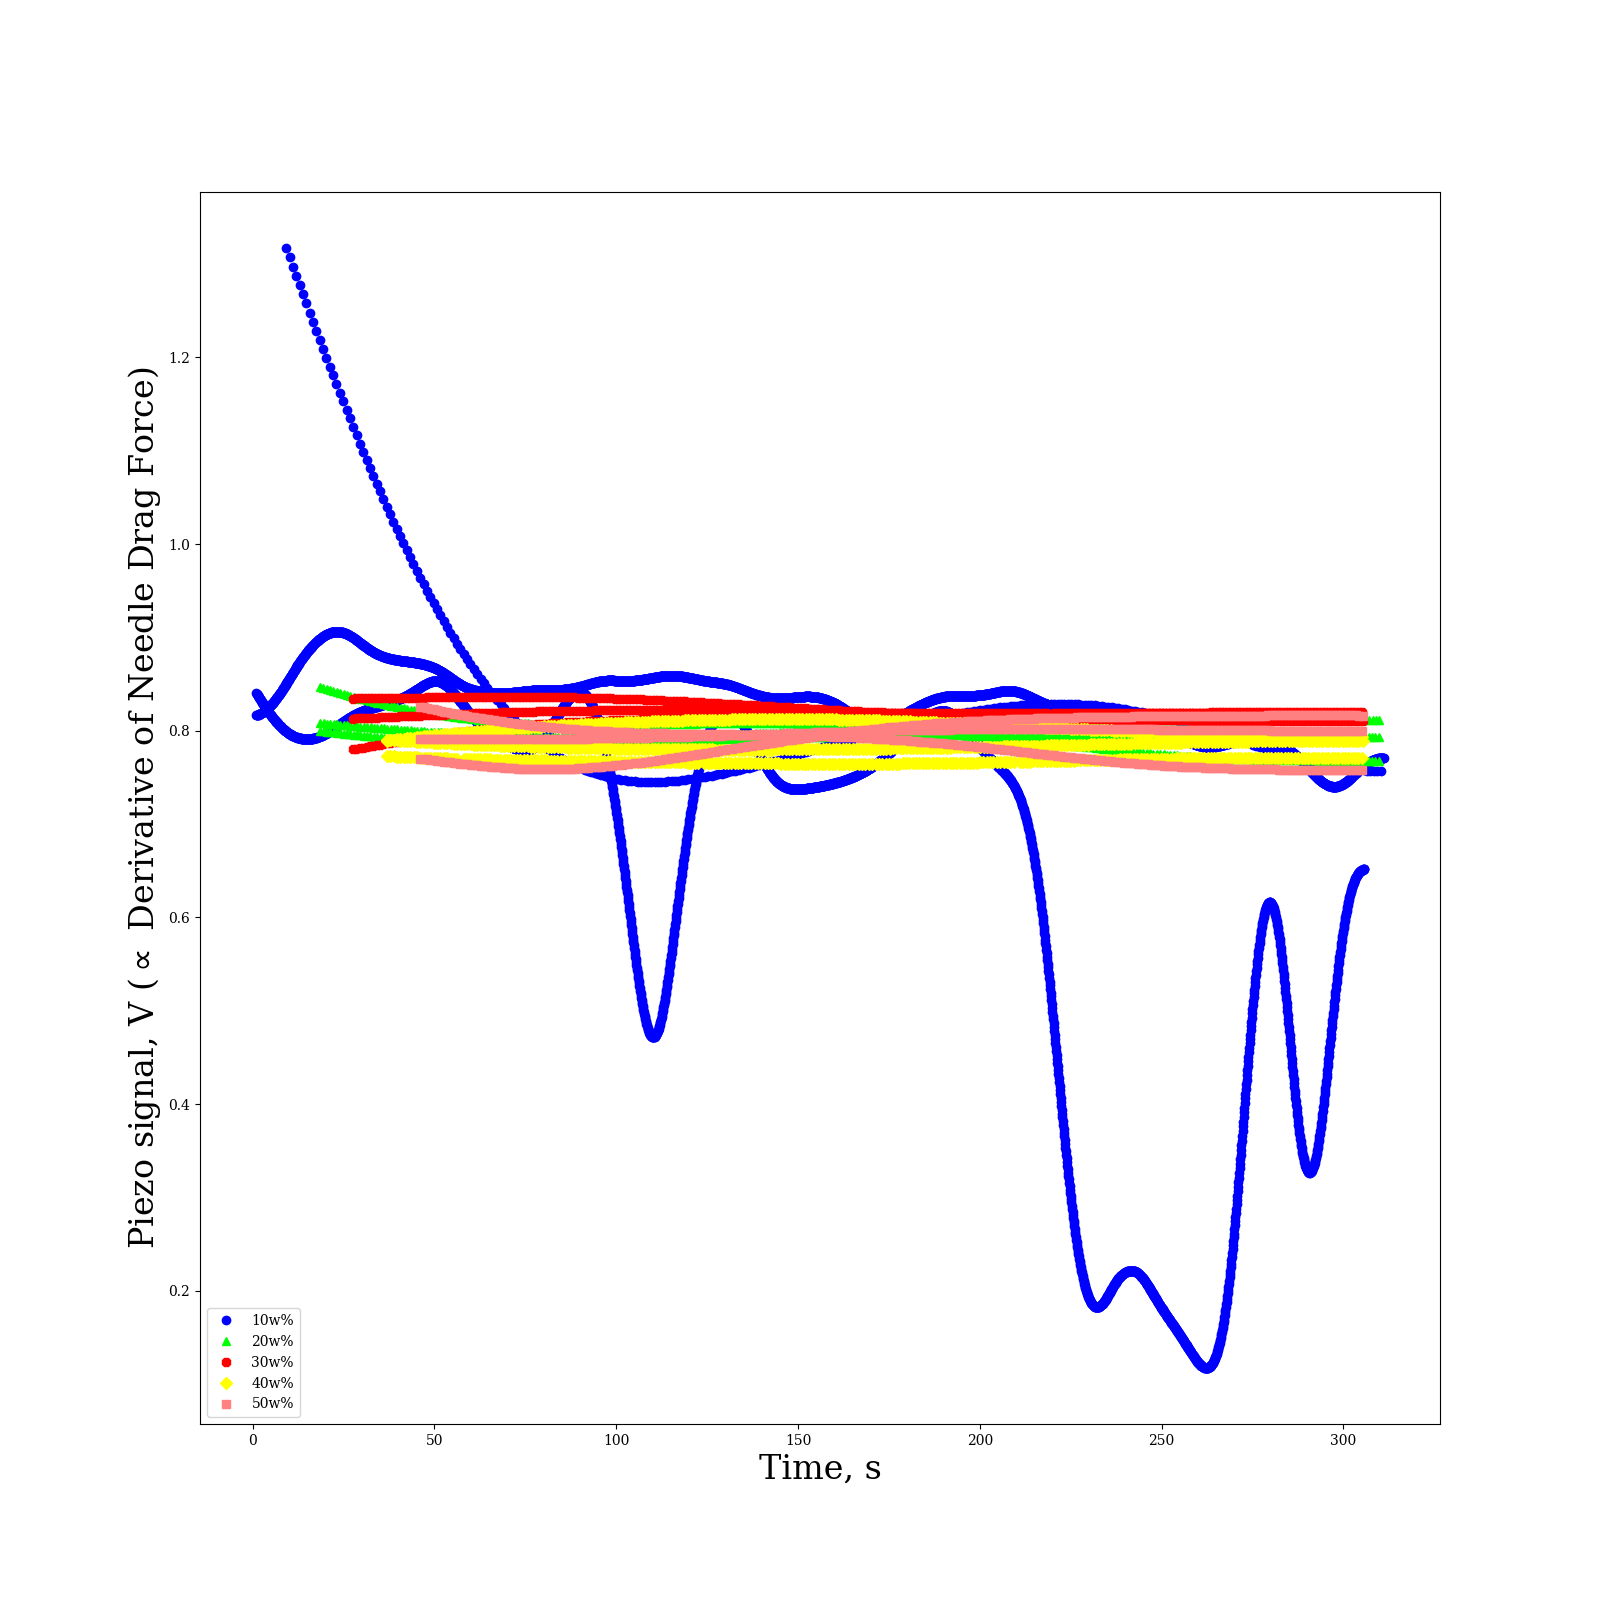
\includegraphics[width=0.4\textwidth]{logs_piezo_compare.png}\\
	\textit{FIG. 3. Raw and Corrected Piezo Plot}\\}
	
\end{document}